{
\renewcommand{\thechapter}{\arabic{chapter}R}
\setcounter{chapter}{15}
\chapter{Exame de recurso 2015/16}
\section{Pergunta 1}
Uma hierarquia de classes representa:
\begin{enumerate}[label=\alph*.]\itemsep0em
    \item Não quero responder
    \item uma associação reflexiva com base na relação de especialização
    \item uma associação com base na relação de agregação
    \item \textbf{um conjunto de classes organizadas com base na relação de especialização \greencheckmark}
    \item um conjunto de classes organizadas com base na relação de composição
\end{enumerate}
Numa hierarquia de classes, a relação distintiva é a especialização (linha contínua com seta aberta branca), não a composição (linha contínua com seta fechada, e losango preto)

\section{Pergunta 2}
A relação \texttt{Empresa(códigoEmpresa, NumeroIdentificaçãoFiscal, NomeEMorada, RamoAtividade)} não está na 1FN porque:
\begin{enumerate}[label=\alph*.]\itemsep0em
    \item nem todos os atributos dependem da chave
    \item nenhuma das outras alternativas porque a relação está na 1FN.
    \item tem duas chaves candidatas
    \item Não quero responder
    \item \textbf{nem todos os atributos são atómicos \greencheckmark}
\end{enumerate}
\texttt{NomeEMorada} não é atómico, dado que semanticamente é composto pelo par \texttt{(Nome, Morada)}.

\section{Pergunta 3}
Qual a expressão em álgebra relacional equivalente à seguinte consulta SQL:
\begin{lstlisting}[language=SQL]
SELECT a FROM T1 JOIN T2 WHERE T1.a > T2.b AND c=-1;
\end{lstlisting}
\begin{enumerate}[label=\alph*.]\itemsep0em
    \item $\sigma_{c=-1 \wedge T1.a > T2.b}(\pi_{a}(T1 \naturaljoin T2))$
    \item $\pi_{a}((\sigma_{c=-1}(T1)) \naturaljoin_{T1.a > T2.b} T2)$
    \item Não quero responder
    \item $\sigma_{c=-1}(\pi_{a}(T1 \naturaljoin_{T1.a > T2.b} T2))$
    \item \textbf{$\pi_{a}(\sigma_{c=-1}(T1 \naturaljoin_{T1.a > T2.b} T2))$ \greencheckmark}
\end{enumerate}
$\pi_{a}(\sigma_{T1.a > T2.b \wedge c=-1}(T1 \naturaljoin T2))$, que é equivalente a $\pi_{a}(\sigma_{c=-1}(T1 \naturaljoin_{T1.a > T2.b} T2))$

\section{Pergunta 4}
Em LDD-SQL, \texttt{FOREIGN KEY} e \texttt{REFERENCES} são
\begin{enumerate}[label=\alph*.]\itemsep0em
    \item a forma de definir uma chave externa e um campo referência, respetivamente
    \item \textbf{duas formas de definir chaves externas \greencheckmark}
    \item duas formas de definir chaves candidatas
    \item Não quero responder
    \item a forma de definir uma chave externa e uma chave candidata, respetivamente
\end{enumerate}

\section{Pergunta 5}
?
\begin{enumerate}[label=\alph*.]\itemsep0em
    \item Não quero responder
    \item só quando se utiliza o \texttt{SELECT}
    \item \textbf{em geral mas ocupa algum espaço em disco \greencheckmark}
    \item sempre
    \item só quando se utiliza o \texttt{UPDATE}
\end{enumerate}

\section{Pergunta 6}
O SQL embebido permite
\begin{enumerate}[label=\alph*.]\itemsep0em
    \item \textbf{a implementação de tarefas parcialmente em SQL e parcialmente na linguagem hospedeira, com troca de informação em variáveis partilhadas \greencheckmark}
    \item Não quero responder
    \item implementação de tarefas totalmente na linguagem hospedeira, que acede à informação de que necessita por referência aos campos das tabelas como variáveis
    \item implementação de tarefas parcialmente em SQL e parcialmente na linguagem hospedeira, com troca de informação por mensagens
    \item implementação de tarefas totalmente na linguagem hospedeira, que acede à informação de que necessita através da execução de comandos em SQL
\end{enumerate}

\section{Pergunta 7}
Um escalonamento recuperável sobre um conjunto de transações
\begin{enumerate}[label=\alph*.]\itemsep0em
    \item não gera bloqueios
    \item garante que a base de dados fica consistente
    \item \textbf{só comete uma transação $T_i$ se as transações $T_j$ cujas alterações foram usadas por $T_i$ já tiverem sido cometidas \greencheckmark}
    \item resulta numa base de dados igual à que seria obtida se as transações fossem executadas em série
    \item Não quero responder
\end{enumerate}

\section{Pergunta 8}
Uma base de dados NoSQL do tipo ``key value store'' consiste:
\begin{enumerate}[label=\alph*.]\itemsep0em
    \item numa estrutura organizada por colunas
    \item em 2 tabelas, uma com as propriedades dos nós e outra com as suas relações
    \item Não quero responder
    \item numa base de dados sem qualquer esquema explícito
    \item \textbf{simplemente numa tabela com 2 colunas, a chave e o valor respetivo \greencheckmark}
\end{enumerate}

\section{Pergunta 9}
O esquema dos dados numa base de dados relacional e num data warehouse é de natureza diferente, nomeadamente relacional e multidimensional:
\begin{enumerate}[label=\alph*.]\itemsep0em
    \item \textbf{mas, tipicamente, são ambas implementadas com software de gestão de bases de dados relacionais \greencheckmark}
    \item tendo, por isso, de ser implementadas com software de bases de dados de tipos diferentes
    \item Não quero responder
    \item sendo, por isso, tipicamente implementadas com software de gestão de bases de dados de tipos diferentes, embora seja possível usar software do mesmo tipo
    \item mas podem ser ambas implementadas com software de gestão de bases de dados relacionais e multidimensionais
\end{enumerate}

\section{Pergunta 10}
Para avaliar a capacidade preditiva de um modelo, é preciso definir os seguintes aspetos:
\begin{enumerate}[label=\alph*.]\itemsep0em
    \item Não quero responder
    \item \textbf{medida de avaliação e forma de utilização dos dados para estimar o valor dessa medida de avaliação \greencheckmark}
    \item algoritmo, medida de avaliação e forma de utilização dos dados para estimar o valor dessa medida de avaliação
    \item algoritmo e medida de avaliação
    \item algoritmo e forma de utilização dos dados para estimar o valor da medida de avaliação
\end{enumerate}

\newpage
\section*{Informação}
Considere o esquema relacional $R(A,B,C,D,E,F,G,H)$ e as seguintes dependências funcionais:
\begin{alignat*}{2}
    & A, B, C && \rightarrow D, G, H \\
    & F       && \rightarrow B, A    \\
    & B       && \rightarrow E       \\
    & D       && \rightarrow H       \\
    & E       && \rightarrow B, C    \\
    & D       && \rightarrow F
\end{alignat*}

\section{Pergunta 11}
Qual das seguintes dependências funcionais não pode ser obtida?
\begin{enumerate}[label=\alph*.]\itemsep0em
    \item \label{itm:2016R-11-a} $A, E \rightarrow G$
    \item \label{itm:2016R-11-b} $B, C, D \rightarrow F$
    \item \label{itm:2016R-11-c} $A,C \rightarrow F,H$
    \item \label{itm:2016R-11-d} $A,C,D \rightarrow F,G$
    \item \label{itm:2016R-11-e} Não quero responder
\end{enumerate}
O item \ref{itm:2016R-11-a} é possível se considerarmos $\{A,E\}^+ = \{A,B,C,E\}^+ = \{A,B,C,D,E,G,H\}^+$.\\
O item \ref{itm:2016R-11-b} é possível se considerarmos $\{B,C,D\}^+ = \{B,C,D,F\}^+$.\\
O item \ref{itm:2016R-11-c} não é possível dado que $\{A,C\}^+ = \{A,C\}$.\\
O item \ref{itm:2016R-11-d} é possível se considerarmos $\{A,C,D\}^+ = \{A,C,D,F\}^+ = \{A,C,D,F,H\}^+$.

\section{Pergunta 12}
Verifique se a relação $R$ se encontra na forma normal de Boyce-Codd. Justifique.

\ansseparator

Uma relação está na forma normal de Boyce-Codd (BCNF) sse, para toda a dependência funcional não-trivial $\overline{A} \rightarrow \overline{B}$, $\overline{A}$ for uma superchave.

Dado que $\{B\}^+ = \{B,E\}^+ = \{B,C,E\}^+ = \{B,C,E\}$, $\{B\}$ não é uma superchave porque o seu fecho não inclui todos os atributos. Assim, a relação $R$ não está na BCNF.

\newpage
\section{Pergunta 13}
Construa um modelo concetual de dados em UML para armazenar a informação associada à realização de uma conferência científica. Indique todas as restrições consideradas importantes para a construção da base de dados.

Os responsáveis pela organização de uma conferência científica pretendem desenvolver um sistema para organizar toda a informação relativa às pessoas envolvidas no evento, às sessões agendadas, às publicações aceites, aos palestrantes convidados, e às revisões associadas a cada publicação.

A organização de uma conferência científica envolve uma comunidade alargada de pessoas que desempenham diferentes papéis, nomeadamente: participantes inscritos na conferência, oradores convidados para a conferência, autores dos artigos e revisores dos artigos. É comum a mesma pessoa desempenhar múltiplos papéis, p.e. um revisor pode ser um autor (de um outro artigo).

Cada pessoa está associada a áreas científicas (p.e. Sistemas de Informação, Computação Gráfica, etc), até um máximo de 3 áreas. Cada pessoa tem sempre um país de origem definido e pode ter ou não definida uma instituição de filiação. Relativamente aos oradores é necessário registar a biografia, bem como a sessão em que participa.

Em relação aos participantes, é necessário registar a data de inscrição, o tipo de inscrição (p.e. estudante, normal, etc) e preço associado.

Os autores estão associados a publicações segundo uma determinada ordem que é necessário registar (1º autor, 2º autor, etc). Relativamente a cada publicação, é necessário registar o título e o resumo, bem como um conjunto de palavras-chave de uma lista pré-definida. Cada publicação tem obrigatoriamente 1 palavra-chave associada até um máximo de 5. Entre os autores de uma publicação, é necessário registar o apresentador do trabalho.

Cada publicação tem também associado um conjunto de revisões feitas pelos revisores. Cada revisor pode rever várias publicações e cada revisão tem uma classificação numérica e uma descrição textual.

Finalmente, pretende-se também registar as sessões da conferência e as salas em que decorrem. Cada sala pode acolher múltiplas sessões. Cada sessão tem uma hora de início, uma hora de fim e um moderador, que é um autor. Cada sessão pode ter associado um orador e um conjunto de publicações a apresentar. Relativamente às publicações a apresentar na sessão é necessário registar a ordem de apresentação.

\ansseparator

\begin{center}
    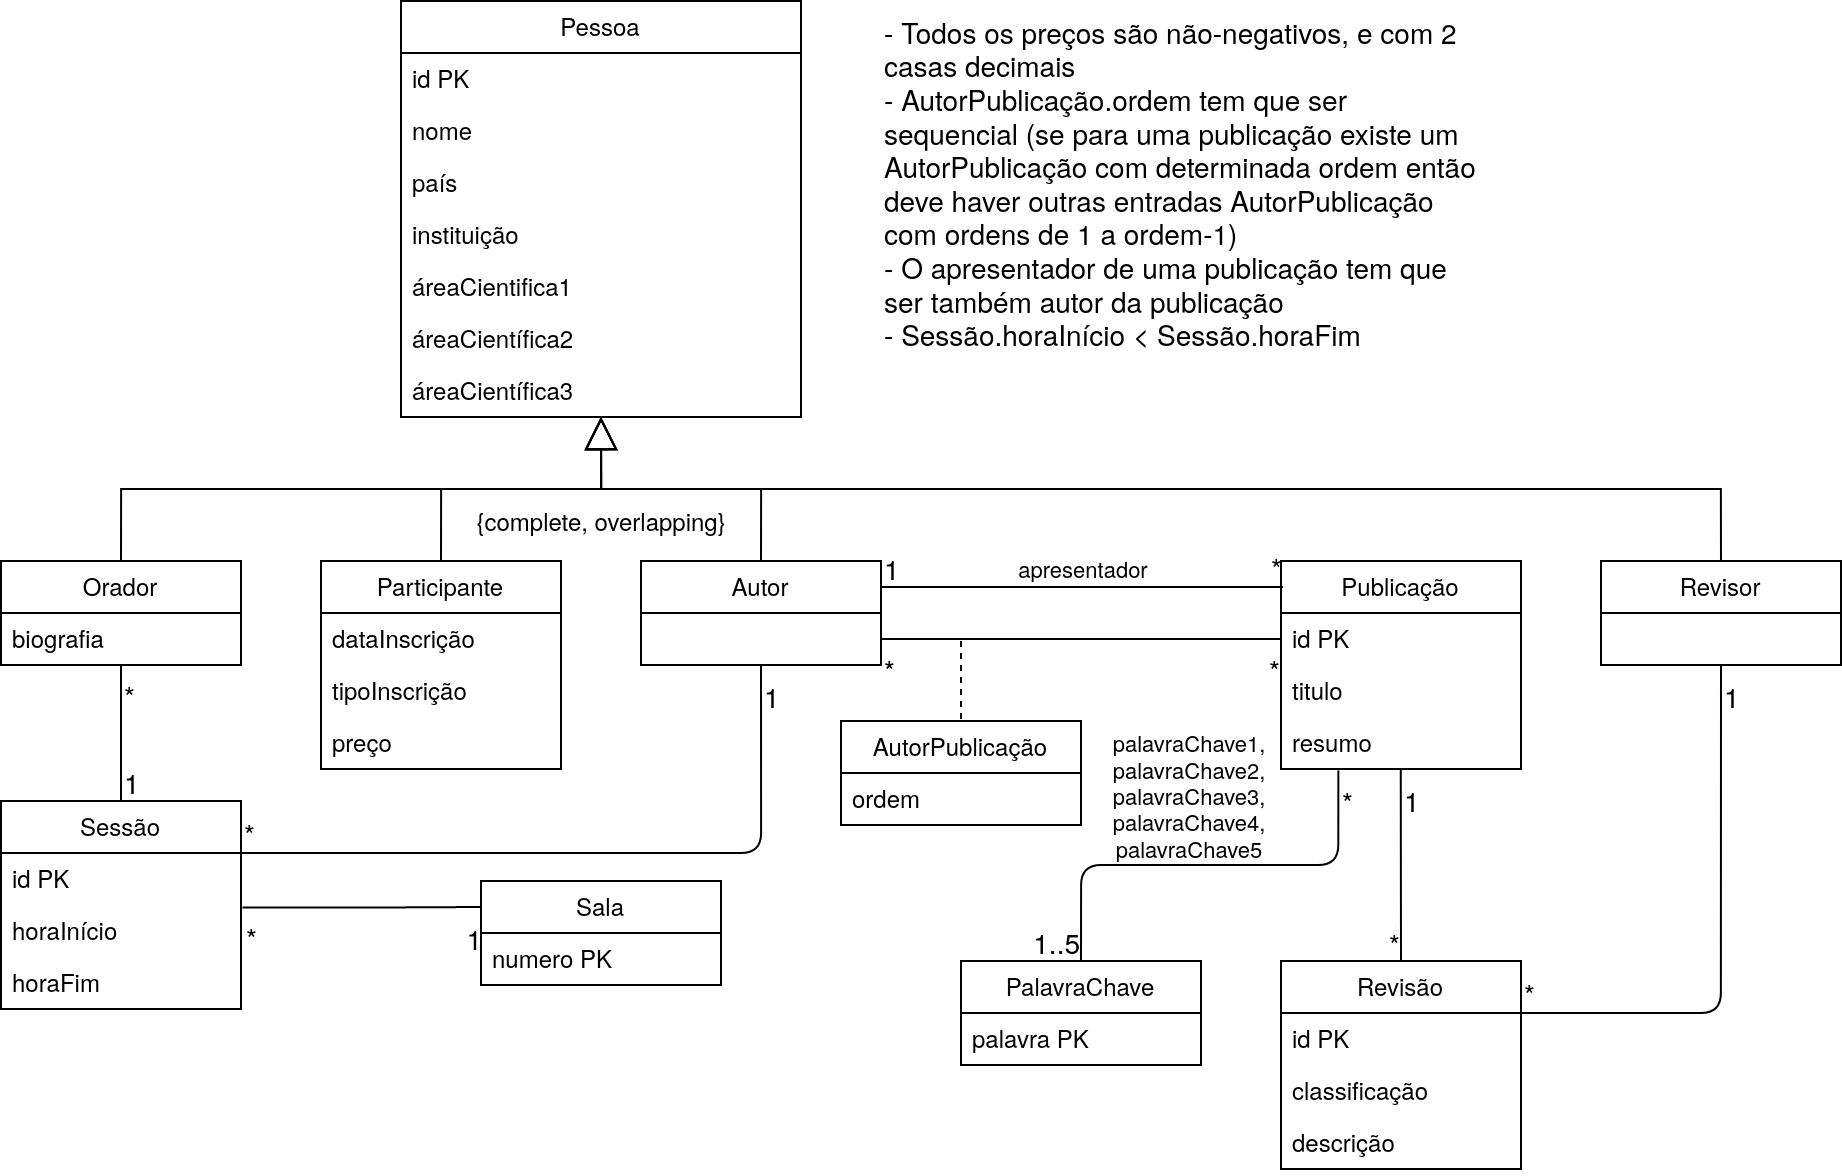
\includegraphics[scale=0.246]{2016R_13.png}
\end{center}

\newpage
\section*{Informação}
Os estudantes da FEUP decidiram organizar a sua rede social usando uma base de dados com o seguinte modelo relacional:

\begin{lstlisting}[numbers=none]
Curso (ID, nome)
Estudante (ID, nome, curso->Curso, anoCurricular)
Amizade (ID1->Estudante. ID2->Estudante)
\end{lstlisting}

O estudante com ID1 é amigo do estudante com ID2. Como as amizades são mútuas, se (176, 9) está na tabela \texttt{Amizade}, (9,176) também está.

A execução das interrogações deve ser feita numa base de dados SQLite criada com as instruções SQL existentes no ficheiro \texttt{redesocial.sql}.

Deve escrever a interrogação usando SQL. Como as interrogações serão executadas usando SQLite, devem ser compatíveis com a sintaxe SQL suportada pelo SQLite.

Para cada interrogação é apresentada a resposta esperada para a base de dados associada ao ficheiro \texttt{redesocial.sql}. Esta informação deve ser utilizada para validar a resposta antes de a submeter. Por omissão, a saída do SQLite só apresenta colunas com 10 caracteres. O número de caracteres de cada coluna pode ser ajustado utilizando o comando:

\begin{lstlisting}[language=SQL,numbers=none]
.width <num caracteres coluna 1> < num caracteres coluna 2>...
\end{lstlisting}

\section{Pergunta 14}
Liste o nome de cada estudante inscrito no MIEIC cujo nome contenha a letra `a'.
\begin{center} \begin{tabular}{l}
    \textbf{Estudante} \\ \hline
    Ana Lopes          \\
    Joao Nunes         \\
    Maria Felisberta   \\
    Cristiano Rodrigo  \\
    Carla Silva        \\
    Carlos Rodrigues   \\
    Mafalda Pimentel   
\end{tabular} \end{center}
\lstinputlisting[language=SQL]{2016R_14.sql}

\section{Pergunta 15}
Liste o nome de todos os estudantes que são amigos de alguém cujo nome comece por Gabriel.
\begin{center} \begin{tabular}{l}
    \textbf{nome}    \\ \hline
    Ana Lopes        \\
    Joana Teixeira   \\
    Mafalda Pimentel \\
    Luis Goncalves   \\
    Barbara Coutinho
\end{tabular} \end{center}
\lstinputlisting[language=SQL]{2016R_15.sql}

\section{Pergunta 16}
Liste o nome dos estudantes com amigos em todos os anos curriculares.
\begin{center} \begin{tabular}{l}
    \textbf{Nome}    \\ \hline
    Gabriel Maria
\end{tabular} \end{center}
\lstinputlisting[language=SQL]{2016R_16.sql}

\newpage
\section{Pergunta 17}
Considere que, para todos os casos em que A é amigo de B e B é amigo de C, A é amigo de C. Crie uma tabela chamada AmizadeTransitiva que contenha estas novas relações de amizade. Não adicione amizades duplicadas, amizades que já existem na tabela Amizade ou auto-amizades.

No final, a tabela AmizadeTransitiva deverá conter os seguintes tuplos:
\begin{center}
    \begin{tabular}{c c c}
        \begin{tabular}{l | l}
            \textbf{ID1} & \textbf{ID2} \\ \hline
            201101025    & 201101304    \\
            201101247    & 201101510    \\
            201101247    & 201101689    \\
            201101247    & 201101934    \\
            201101304    & 201101025    \\
            201101304    & 201101316    \\
            201101304    & 201101501    \\
            201101304    & 201101510    \\
            201101304    & 201101709    \\
            201101316    & 201101304    \\
            201101316    & 201101501    \\
            201101316    & 201101510    \\
            201101316    & 201101709    \\
            201101381    & 201101501    \\
            201101381    & 201101689    \\
            201101381    & 201101709    \\
            201101381    & 201101911    \\
            201101501    & 201101304    \\
            201101501    & 201101316    \\
            201101501    & 201101381    \\
            201101501    & 201101709    \\
            201101510    & 201101247    \\
            201101510    & 201101304    \\
            201101510    & 201101316    \\
            201101510    & 201101709    \\
            201101510    & 201101782
        \end{tabular}
        & &
        \begin{tabular}{l | l}
            \textbf{ID1} (cont.) & \textbf{ID2} (cont.) \\ \hline
            201101661    & 201101689    \\
            201101661    & 201101782    \\
            201101661    & 201101934    \\
            201101689    & 201101247    \\
            201101689    & 201101381    \\
            201101689    & 201101661    \\
            201101689    & 201101934    \\
            201101709    & 201101304    \\
            201101709    & 201101316    \\
            201101709    & 201101381    \\
            201101709    & 201101501    \\
            201101709    & 201101510    \\
            201101709    & 201101782    \\
            201101709    & 201101911    \\
            201101782    & 201101510    \\
            201101782    & 201101661    \\
            201101782    & 201101709    \\
            201101782    & 201101934    \\
            201101911    & 201101381    \\
            201101911    & 201101709    \\
            201101911    & 201101934    \\
            201101934    & 201101247    \\
            201101934    & 201101661    \\
            201101934    & 201101689    \\
            201101934    & 201101782    \\
            201101934    & 201101911
        \end{tabular}
    \end{tabular}
\end{center}
\lstinputlisting[language=SQL]{2016R_17.sql}

\newpage
\section{Pergunta 18}
Liste todos os pares de amigos de cursos diferentes. A listagem não deve conter pares repetidos, nem pares simétricos. Se contiver o par (Miguel, Nuno) não deve ter o par (Nuno, Miguel).
\begin{center} \begin{tabular}{l l}
    \textbf{Nome}    & \textbf{Nome}    \\ \hline
    Ana Lopes        & Gabriel Maria    \\
    Maria Felisberta & Diogo Teixeira   \\
    Carla Silva      & Sergio Carvalho  \\
    Sergio Carvalho  & Pedro Nunes      \\
    Joana Teixeira   & Pedro Nunes      \\
    Mafalda Pimentel & Cristina Ribeiro \\
    Mafalda Pimentel & Gabriel Maria    \\
    Carla Silva      & Luis Gonçalves   \\
    Mafalda Pimentel & Barbara Coutinho \\
    Sergio Carvalho  & Carlos Rodrigues
\end{tabular} \end{center}
\lstinputlisting[language=SQL]{2016R_18.sql}

\section{Pergunta 19}
Crie os gatilhos necessários para garantir que a amizade é mútua sempre que haja inserções ou eliminações na tabela \texttt{Amizade}. Crie também um gatilho que impeça atualizações à tabela \texttt{Amizade}.
\lstinputlisting[language=SQL]{2016R_19.sql}

}
